\documentclass[10pt,twocolumn,letterpaper]{article}

\usepackage{cvpr}
\usepackage{times}
\usepackage{epsfig}
\usepackage{graphicx}
\usepackage{amsmath}
\usepackage{amssymb}

% Include other packages here, before hyperref.

% If you comment hyperref and then uncomment it, you should delete
% egpaper.aux before re-running latex.  (Or just hit 'q' on the first latex
% run, let it finish, and you should be clear).
\usepackage[breaklinks=true,bookmarks=false]{hyperref}

\cvprfinalcopy % *** Uncomment this line for the final submission

\def\cvprPaperID{****} % *** Enter the CVPR Paper ID here
\def\httilde{\mbox{\tt\raisebox{-.5ex}{\symbol{126}}}}

% Pages are numbered in submission mode, and unnumbered in camera-ready
%\ifcvprfinal\pagestyle{empty}\fi
\setcounter{page}{4321}
\begin{document}

%%%%%%%%% TITLE
\title{Vision and Language in 3D}

\author{Yuval Atzmon\\
Bar Ilan University\\
Ramat Gan, Israel\\
{\tt\small yuval.atzmon@biu.ac.il}
% For a paper whose authors are all at the same institution,
% omit the following lines up until the closing ``}''.
% Additional authors and addresses can be added with ``\and'',
% just like the second author.
% To save space, use either the email address or home page, not both
\and
Alessia Vignolo\\
DIBRIS and IIT\\
Genova, Italy\\
{\tt\small alessia.vignolo@gmail.com}
}

\maketitle
%\thispagestyle{empty}

%%%%%%%%% ABSTRACT
\begin{abstract}
 We constructed a system that tracks activities in videos, given a descriptive text sentence, and outputs the likelihood of how well the description matches the activity in the video. We integrated depth estimation for single-lens camera and demonstrated its ability to track 3D actions in single-lens camera videos. Actions that could not be otherwise addressed. 
 

\end{abstract}

%%%%%%%%% BODY TEXT
\section{Introduction}

Understanding complex visual scenes, has many aspects: inferring the structure of the scene, detecting and labeling objects, recognizing people, their actions and their interactions, retrieving an image or video given a description, image generation from captions, automatic caption generation and telling the story shown at the scene.

In the past few years, the task of image classification has taken a huge leap in performance, achieving near-human-level accuracy \cite{imagenetHistory, krizhevsky2012imagenet, googlenet}. It was combined with object detection algorithms to generate objects class proposals given a visual image scene \cite{googlenet, girshick2014rcnn}. The main drawback of these approaches is that they avoid the problem of understanding the structure withing a scene and do not take into account the relationship between objects and their attributes in a scene. Current state-of-the-art approaches mostly rely on low level cues and moving search windows to identify objects suggestions and lack a probabilistic framework for understanding the scenes structure, such as understanding that a dog is chasing a human, rather than a human is chasing a dog.

In this work we followed the approach of \cite{siddharth2014seeing}, which provides a medium for a multimodal integration of vision and language in videos. This approach uses the textual description and grammar as top-down prior for detection and understanding interactions, and integrates it with bottom-up object proposals and optical flow inference. We integrated depth estimation \cite{depthfayao} for single-lens camera, and demonstrated its ability to track 3D actions in single-lens camera videos. Actions that could not be otherwise addressed. 



\begin{figure}[ht]
\begin{center}
%\fbox{\rule{0pt}{2in} \rule{0.9\linewidth}{0pt}}
   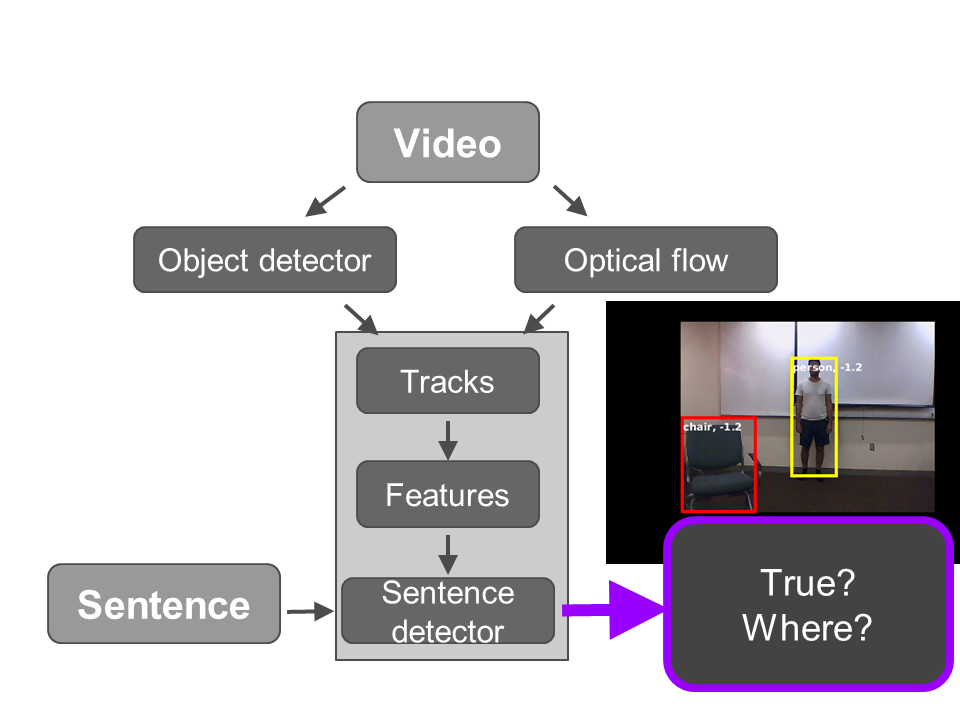
\includegraphics[width=0.8\linewidth]{system_overview.png}
\end{center}
   \caption{System overview}
\label{fig_system}
\end{figure}

\section{Vision and language system}

The system is composed of several blocks which run simultaneously (an overview is shown in Figure \ref{fig_system}): it takes a single-lens camera video and a sentence as input and says if the event described in the sentence is in the video and where it happens.\\
Starting from a video, we run an object detector on each frame, allowing many false-positives and, therefore, a high detection rate. We use the detections as states of a generalized Hidden Markov Model (HMM) of a tracker that gives high score for coherency between frames (we use optical flow to account for movement), and do inference over it by solving a dynamic programming problem with a Viterbi decoder \cite{viterbi}, to find the best track.
The HMM has a second layer, related to the meaning of the sentence, which biases the tracker results accordingly. In practice, we match a tracker for each noun of the sentence, and do joint inference on the states of the video trackers and the language HMM model all together. As an example, a sentence composed by a verb and two nouns ("A person approaches a chair") will generate two trackers, one for each noun. The observations of the 1st noun will be classes of detections of the 1st tracker; the observations of the 2nd noun will be classes of detections of the 2nd tracker and the observations of verb will be features of the detections of both trackers (e.g. the relative distances and velocities between them).
We take the outer product of all possible states of all the HMMs and combine them into a single Viterbi inference mechanism. Eventually, the system results with tracking only the actions that were described in the sentence (implementing a sort of an attention mechanism), and returning a likelihood score for how well this action corresponds to the events in the video. 

%-------------------------------------------------------------------------
\subsection{Integrating depth estimation}
In order to track the actions performed in a perpendicular direction with respect to the camera plane, the 3D information of the depth is needed.
Several state-of-the-art systems allow to extract the 3D information, like kinect sensors and stereo vision system. Instead, we chose to use a multi-scale deep network which is able to perceive depth for single-lens camera images \cite{depthfayao}. The network was trained on samples of RGB images with and depth information as a supervision signal. The package is available online \cite{depthfayao} and an example of the output for depth estimation is in Figure \ref{fig_depth_frame}.
The vision and language system can now be improved by extracting the features, which are relevant in the definition of the verb in the sentence (e.g. relative position, velocity etc.) in a 3D coordinate system instead of a 2D one, enabling the system to track also the movements towards the camera.

\section{Results}
We acquired two videos where a person approaches a chair: in one case, the action is performed along a parallel direction with respect to the camera plane (Figure \ref{fig_front_vs_side}, left) and, in the other case, along a perpendicular direction (Figure \ref{fig_front_vs_side}, right). Then, we compared the performance of the 2D system and the 3D one on both the videos, computing the likelihood scores which says how well the sentence "A person approaches a chair" matches the activity in the video. 
Table \ref{table_likelihood} shows the likelihood scores of textual descriptions in videos of frontal approach and side approach, while comparing 2D inference \cite{siddharth2014seeing} vs 3D inference (ours): in the case of a movement parallel to the camera plane, both systems are reliable. In the case of a movement perpendicular to the camera plane, the 2D system fails, while the 3D system is still able to match the sentence with the event happening in the video giving a high likelihood score.



\begin{figure}[ht]
\begin{center}
%\fbox{\rule{0pt}{2in} \rule{.9\linewidth}{0pt}}
   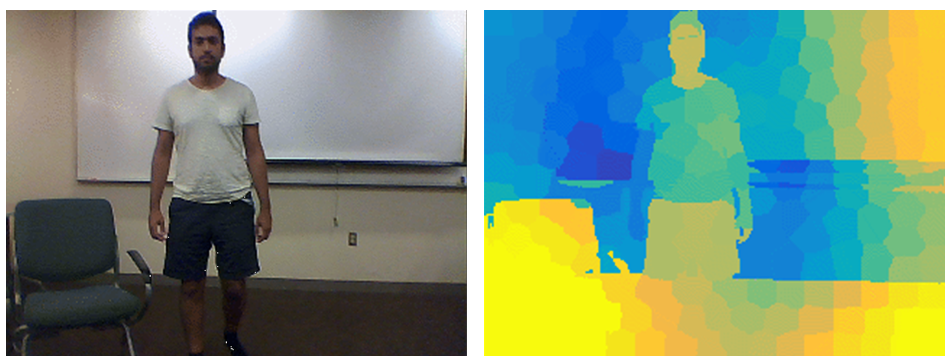
\includegraphics[width=0.8\linewidth]{depth_estim_example.png}
   \end{center}
   \caption{Example for depth estimation in a single frame, bright yellows denote smaller depths, dark blues denote larger depths.}
\label{fig_depth_frame}
\end{figure}

\begin{figure}[ht]
\begin{center}
%\fbox{\rule{0pt}{2in} \rule{.9\linewidth}{0pt}}
   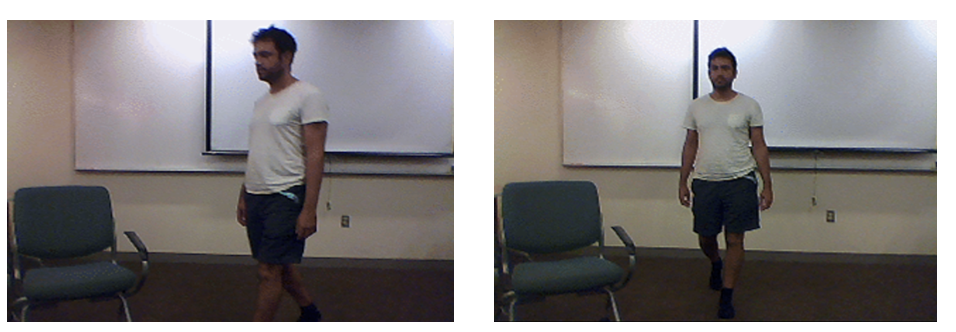
\includegraphics[width=0.8\linewidth]{front_vs_side_approach.png}
   \end{center}
   \caption{"A person approaches a chair": side vs frontal approach}
\label{fig_front_vs_side}
\end{figure}

\begin{table}
\begin{center}
\begin{tabular}{|l|c|c|}
\hline 
 Log likelihood & Side approach & Frontal approach  \\
\hline\hline
3D (ours) & -43 & -50\\
2D \cite{siddharth2014seeing} & -10 & -1020 \\
\hline
\end{tabular}
\end{center}
\caption{Log likelihood scores of textual descriptions in videos of frontal approach and side approach for \textit{
"A person approaches a chair"}. Comparing 2D inference \cite{siddharth2014seeing} versus 3D inference (ours), we see that the 2D system fails (very low likelihood score) when the action requires perceiving the depth.}
\label{table_likelihood}
\end{table}

{\small
\bibliographystyle{unsrt} % Sort the bibliography by citation order
\bibliographystyle{ieee}
\bibliography{references}
}

\end{document}
